%第15章
\chapter{指对数}
\href{https://en.wikipedia.org/wiki/John_Napier}{John Napier}在其1614年的巨著《Mirifici logarithmorum canonis descriptio》当中详细地阐述了对数运算的定义,性质等。从此在数学运算当中再也没有任何大数字了,因为这个数字取完对数之后就以几何般的速度下降。
\begin{figure}[H]
\centering
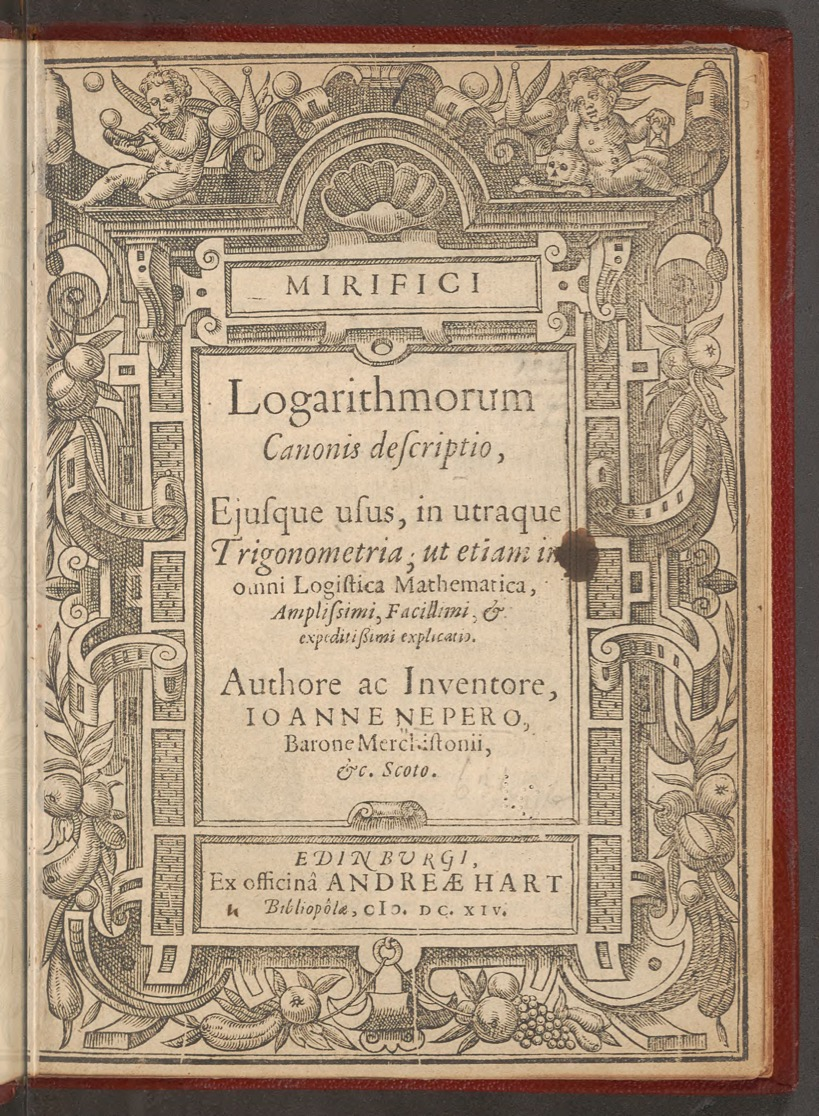
\includegraphics[width=0.5\textwidth]{napier}
\caption{该书的影印版,拉丁原文}
\end{figure}

\section*{学习目标}
\begin{todolist}
 \item 理解对数运算的意义,与指数运算的关系
 \item 掌握并利用对数运算的法则
 \item 不要求掌握换底公式,但是我要求
 \item 绘制指数函数$e^x$以及对数函数$\ln x$的图像,描述两者的关系
 \item 利用对数,解决未知数在指数部分的方程或者不等式
 \item 利用对数做线性化,并根据斜率或者截距求算信息
\end{todolist}
\clearpage

\section{对数}
首先回顾一下指数的定义:
\[
	a^{\boxed{n}}=b
\]

其中$a$称之为为\gls{base},$n$称之为\gls{expo}。比如 $3^4=81$。那么既然可以计底数的$n$次方之后的结果,那么必定也能够逆向地求算\textbf{一个数是底数的多少次方}。这种运算被称之为\gls{log},计作:
\[
	n=\log_a b
\]
读作 n is the logarithm of b to base a
。

因此指数运算和对数运算,就像乘法和除法一样,互为对方的逆运算。$\log$只是为了告诉人们,这是求算次幂的运算,真正想要求算取对数的过程是非常复杂的,我做作为一个普通人,只能记得住常规的整数幂次的求算结果。

\begin{TaskBox}
完成以下常见底数的幂次运算和取对数运算
\begin{table}[H]
\centering
\begin{tblr}{
	colspec={|l|c|c|c|c|c|c|c|c|c|c|},
	}
\hline
exponents& 1 & 2 & 3 & 4 & 5 & 6  & 7 & 8 & 9 & 10\\
\hline
2   &   &	& 8	&	&	&	&	&	&	& 	\\
\hline
logarithm  &   & 4	& 	&	&	&	&	&	&	& 1024 \\
\hline
$\log_2$  	&   & 2	& 	&	&	&	&	&	&	& 10\\
\hline
\end{tblr}
\end{table}

\end{TaskBox}

\subsubsection*{对数运算的法则}
由于指数运算的性质,结合对数运算的逆运算性质,有以下的法则可以使用:\\

\begin{matrix}
$\log_a 1=0$  & $\log_a m+\log_a n =\log_a (m\times n)$ &$\log_a m-\log_a n =\log_a (\frac{m}{n})$\\

$\log_a {\frac{1}{n}} = -\log_a n$ & $\log_a {(m^n)}=n\times \log_a m$ & $\log_{a^n} b=\frac{1}{n}\log_a b$\\

$\log_{a^n} b^m=\frac{m}{n}\times \log_a b$ & $\log_a b=\frac{1}{\log_b a} & a^{\log_a^ m} = m$
\end{matrix}


\begin{ExampleBox}
证明对数运算中$\log_a m+\log_a n =\log_a (m\times n)$
\tcblower
假设 $\log_a m=\bigtriangleup $, $\log_a n=\square$。根据对数的定义。那么$m=a^{\bigtriangleup}, n=a^{\square}$\\
$LHS = \log_a m+\log_a n =\bigtriangleup+\square $\\
$RHS = \log_a (mn)=\log_a (a^{\bigtriangleup}\cdot a^{\square})=log_a (a^{\bigtriangleup+\square})=\bigtriangleup+\square$
所以左右侧相等。
\end{ExampleBox}

\begin{TaskBox}
证明运算法则其他的公式
\end{TaskBox}

\subsection*{不需要掌握的换底公式}
这是对数运算中非常重要的一个性质,但是在A-Level里面不需要掌握。不过还是建议各位了解。叫做\gls{changebase}
\[
	\log_a b=\frac{\log_c b}{\log_c a}
\]
这个公式及其重要,因为,我们可以将任意形式的对数,转变为固定的相同的底$c$。用两者的商来代表$\log_a b$。就有点像早期的三角函数表一样,人们只要研究特定的底数的结果,形成一张对数表,就无需再真正去计算任意对数结果,只需要查表就好了,再做除法就好了。

而有两个数字非常幸运,被选作对数表的基础底数,分别是$10$以及更为牛逼的\gls{Euler's number}——$e\approx 2.718281828459045\ldots$。如果是以$e$为底数,这样的对数一般记错$\ln b$,无需写作$\log_e b$。

\begin{figure}[H]
\centering
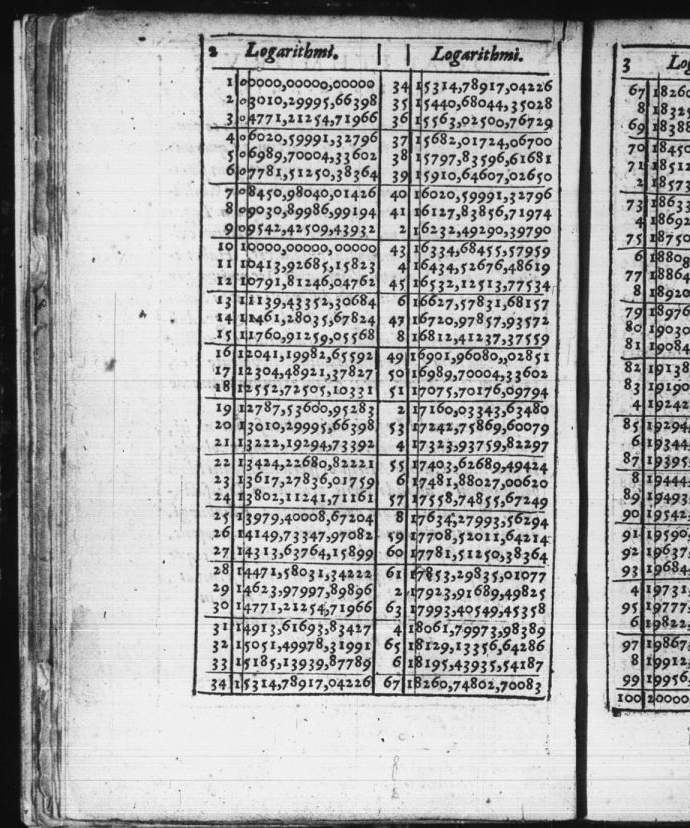
\includegraphics[width=0.8\textwidth]{logtable}
\caption{Briggs计算出以$10$为底,从$1$到$100$的对数表,精确到小数点后14位}
\end{figure}

从上表中不难发现,任何的大数字都可以通过取对数,变成较小的数字,而且不管数字再大也不怕。因而人们根据对数的这些运算性质发明了对数尺,作为一种计算器,方便地求算乘除法和次幂。
\begin{figure}[H]
\centering
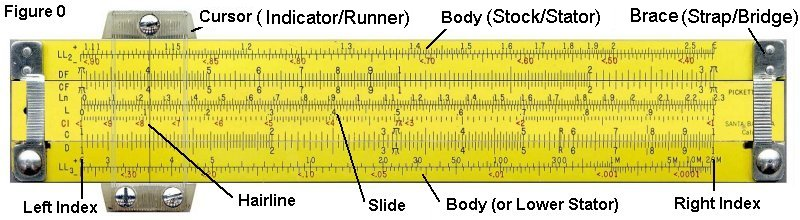
\includegraphics[width=0.8\textwidth]{slide ruler}
\end{figure}

尝试通过移动对数尺上的\href{http://www.antiquark.com/sliderule/sim/n909es/virtual-n909-es.html}{划片}求算 $2.3 \times 3.4 $的\href{https://sliderulemuseum.com/SR_Course.htm}{结果}
\clearpage

\section{指数函数与对数函数}
基础的指数函数$y=a^x$的函数图像为:
\begin{figure}[H]
\centering
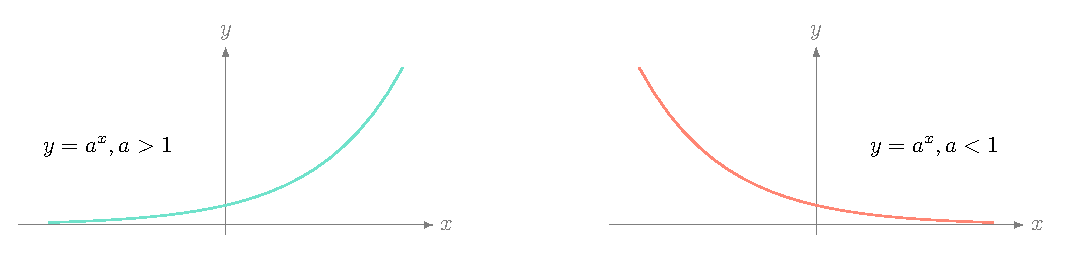
\includegraphics[width=0.8\textwidth]{expo.pdf}
\caption{递增式和递减式的指数函数图像}
\end{figure}

\subsection*{指数函数图像的变形}
不过稍作复杂一点,处理一下$y=A\cdot a^{kx} +C$这种复杂的指数图像。

\subsubsection*{$k$的拉伸/换底作用}
由于这里的$k$会使得指数图像进行水平方向上的拉伸或者压缩,详见\ref{subsec:Stretch}。当然,也可以利用指数运算的性质,将$a^{kx}=(a^k)^x$。也就是将$a^k$作为新的底。

\subsubsection*{$A$的拉伸/水平平移作用}
很明显$A$会使得图像进行竖直方向上的拉升或者压缩,但是由于指数的性质,现在我们将$A$改写为$a^{\left(\log_a A\right)}$。因此有:
\[
	A\cdot a^x =a^{\left(\log_a A\right)}\cdot a^x = a^{\left(x+\log_a A\right)}
\]
因此,等同于将函数图像沿着\emph{水平方向}进行平移,详见\ref{subsec:Translation}。这种性质是指数函数独有的。

同时,$y$-intercept也会从$(0,1)$变成$(0,A)$

\subsubsection*{$C$的平移/渐近线作用}
最后处理$C$,由于在完成指数运算和乘法之后再$+C$,因此会带来\emph{竖直}方向的移动。可以利用\emph{上加下减}的性质进行确认。不过最明显的还是指数图像的\gls{asymptote}。之前的基本渐近线都是$y=0$。无论进行水平还是竖直方向的拉伸都不会改变,但是当整体$+C$之后,渐近线就变成了$y=C$。因此只有这种变形会带来渐近线的改变。

同时$y$-intercept也会从$(0,A)$变成$(0,A+C)$

\begin{SummBox}
在此\href{https://www.desmos.com/calculator/qsbdrninpd}{desmos}中有这三个参数$A,k,C$的模拟演示,自己可以滑动验证
\begin{figure}[H]
\centering
\includegraphics[width=0.8\textwidth]{transformexpo}
\caption{注意指数函数图像的参数变化对截距和渐近线的影响}
\end{figure}
\end{SummBox}


\subsection*{对数函数的图像}
在本阶段中,只需要绘制基础的$y=\log_a x$的图像就足够了,掌握定义域,值域和渐进线就行。
由于指数函数和对数函数互为反函数的性质存在,因此完全符合\ref{subsec:Graphic Charcteristic}所提及的内容。函数图像关于$y=x$对称。如下图所示:
\begin{figure}[H]
\centering
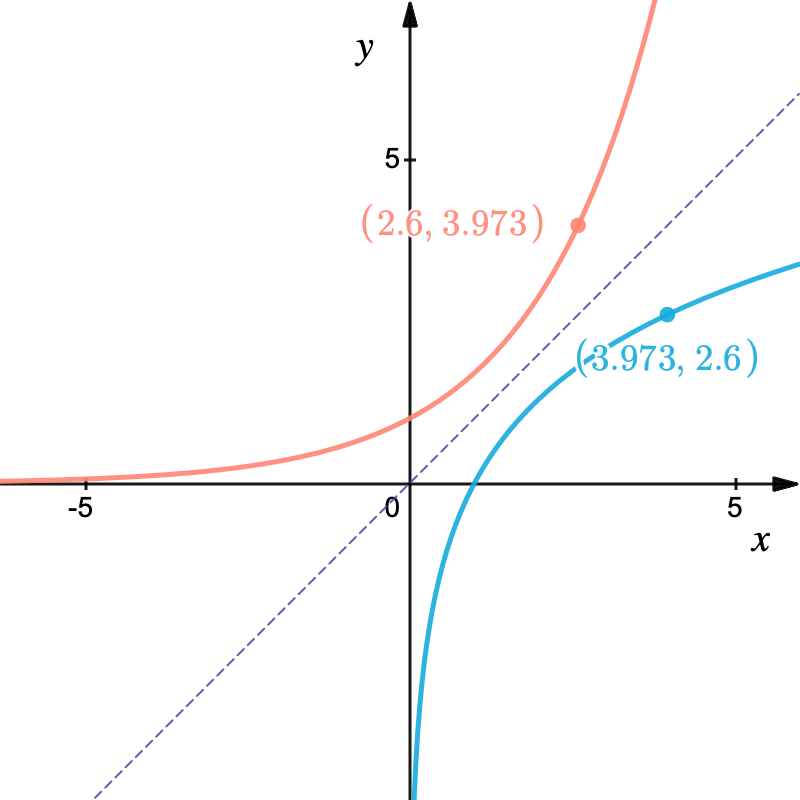
\includegraphics[width=0.4\textwidth]{expolog-in}
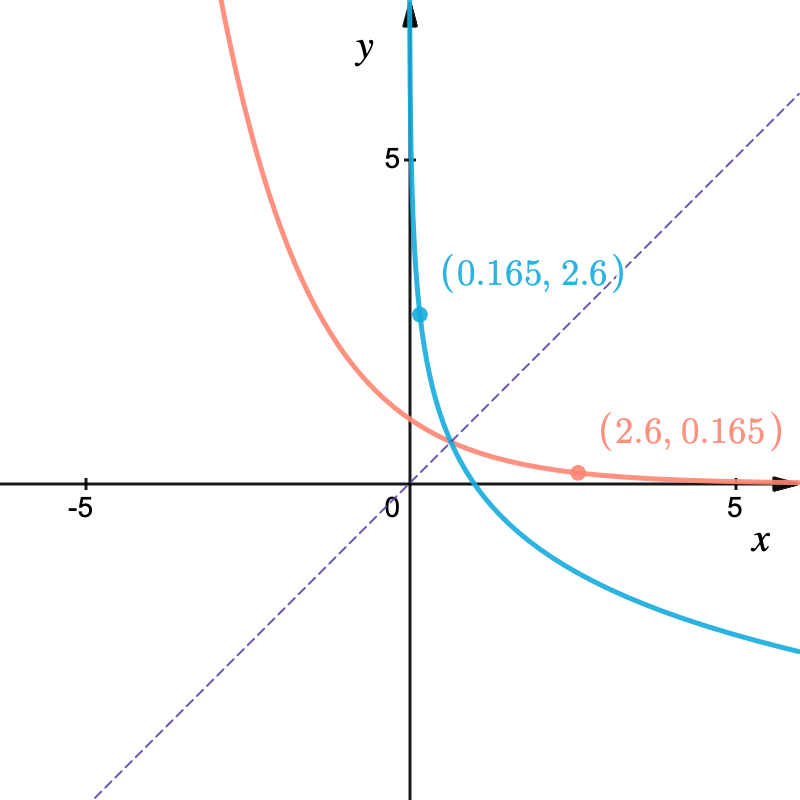
\includegraphics[width=0.4\textwidth]{expolog-de}
\caption{只要确保底数一致,指对数函数图像完全对称}
\end{figure}

因此对于对数函数而言:
\begin{enumerate}[(1)]
\item 定义域为$[0,+\infty)$,或者说 $x>0$;
\item 值域为$(-\infty,+\infty)$,或者说 $y\in \mathcal{R}$;
\item 渐近线变成了$y$轴,或者说 $x=0$
\item 对数函数是一对一函数,有且仅有唯一函数值
\end{enumerate}
这些性质都是从对应的指数函数中推导出来的。
\clearpage

\section{解决含有指数或者对数方程}
在学完指对数的运算之后,再来求解一些含有指对数的方程。比如
\begin{ExampleBox}
solve the equation:$2=\ln (1-x) -\ln x$\\
\makebox{}\hfill adapted from $2017$ summer qp$31$ Q$3$
\tcblower
需要利用指数运算的各种性质去化简
\begin{align*}
 	 2 &= \ln \left(\frac{1-x}{x}\right)\\
 	 e^2 &= \frac{1-x}{x} \\
 	 e^2\cdot x &= 1-x\\
 	 (1+e^2) \cdot x &=1\\
 	  x &=\frac{1}{1+e^2}
\end{align*}
\end{ExampleBox}

或者再看一道例题:
\begin{ExampleBox}
solve for $3^{x+4}=5^{x+1}$
\tcblower
对于这样的函数需要两边同时取对数,底数是3是5都可以,甚至选择任意数字都可以,比如$e, 10, 2$这些
\begin{align*}
 \log_3 {\left(3^{x+4}\right)} &=\log_3 {\left(5^{x+1}\right)}\\
 x+4 &=(x+1)\cdot \log_3 5\\
 4-\log_3 5 &=(\log_3 5-1)\cdot x\\
 x &=\frac{4-\log_3 5}{\log_3 5-1}\\
   &=\frac{\log_3 {\frac{81}{5}}}{\log_3 {\frac{5}{3}}}\\
   &=\log_{\frac{5}{3}} {\frac{81}{5}}\\
   &\approx 5.452
\end{align*}
尝试用$\ln$或者$\log_5$解决此题
\end{ExampleBox}
\clearpage


\section{线性化}
对于生活中存在的指数关系,可以通过取对数的方式变形为对数的线性关系。
\[
	y=ab^x \qquad \text{or} \qquad y=ax^n
\]
对于这样的关系,两边同时取其自然对数,可以得到以下的结果:
\[
	\ln y=\ln a+ x\cdot \ln b \qquad \text{or} \qquad y=\ln a+ n\cdot \ln x
\]

这样的话,重新绘制散点图,但是以$\ln y$的值作为纵坐标,以$x$的值作为横坐标,就能得到直线图像,斜率为$\ln b$ 截距为$\ln a$这种过程就被称之为线性化。

如下图:
\begin{figure}[H]
\centering
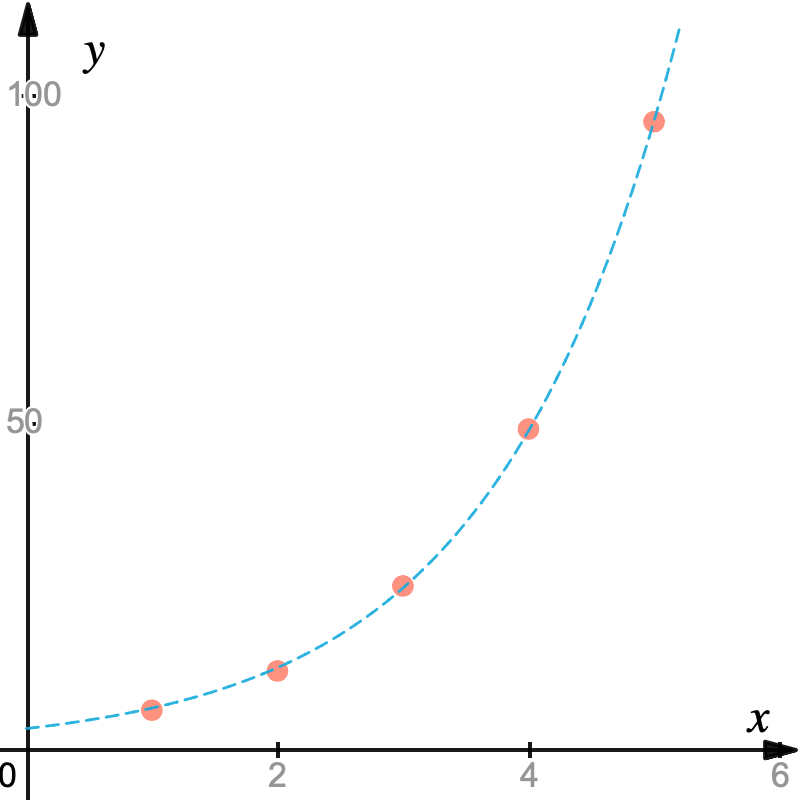
\includegraphics[width=0.4\textwidth]{exporelation}
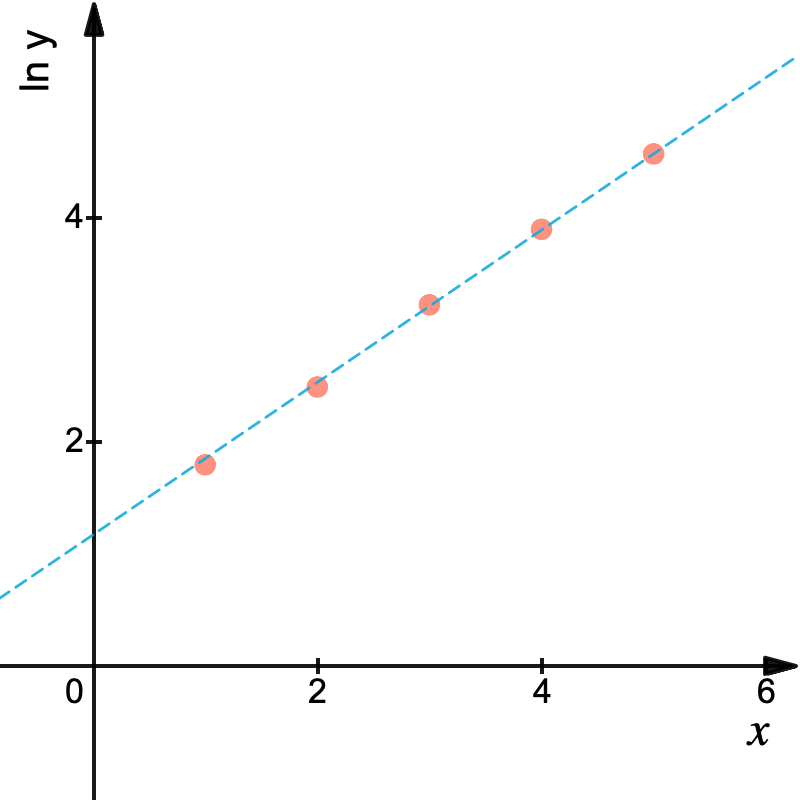
\includegraphics[width=0.4\textwidth]{linearrelation}
\caption{调整数值后得到线性关系}
\end{figure}

\begin{TaskBox}
对于第二个关系,应该以谁作为自变量?才能得到直线关系
\end{TaskBox}

做线性化一般发生在真实的科学研究中,探究的自变量和因变量之间呈现曲线关系的时候,多种函数都能拟合出曲线特征,但是直线式的函数关系就只有唯一的一种。因此可以用来检验研究人员的猜想是否正确。

